\textbf{Целью пятой лабораторной работы} является освоение возможностей программы Microsoft Project по управлению финансовыми потоками на основе анализа затрат.

\section*{Содержание проекта}

Команда разработчиков из 16 человек занимается созданием карты города на основе собственного модуля отображения. Проект должен быть завершен в течение шести месяцев. Бюджет проекта: 50 000 рублей.

\section*{Сведения об актуализированном состоянии проекта}

По состоянию на дату отчета 23.05.2023 в проекте произошли следующие изменения:

\begin{itemize}
	\item задача <<Создание заставки>> закончилась на пять дней позже;
	\item задача <<Программирование средств обработки базы объектов>> закончилась на семь дней раньше;
	\item задача <<Создание мультимедиа-наполнения>> выполнена на 75 \%;
	\item 24.03.2023 уволили ведущего программиста;
	\item с 1.04.2023 подняли заработную плату программистам 1-4 на 20\%;
	\item с 1.04.2023 аренда сервера подорожала на 15\%;
	\item с 1.04.2023 начали проводиться презентации раз в две недели по часу, для каждого из которых нужна пачка бумаги стоимостью 100 рублей;
	\item с 1.04.2023 в еженедельных совещаниях стали принимать участие только те сотрудники, у которых есть задачи на текущей неделе.
\end{itemize}

Состояние остальных задач соответствует базовому плану проекта.

После актуализации проекта отклонение по затратам составило 2 794.14 рублей, отклонение по длительности --- 19 дней, что показано на рисунке \ref{img:deviation1}. При этом, длительность проекта удовлетворяет заявленному сроку, но затраты проекта не умещаются в бюджет.

\begin{figure}[H]
	\begin{center}
		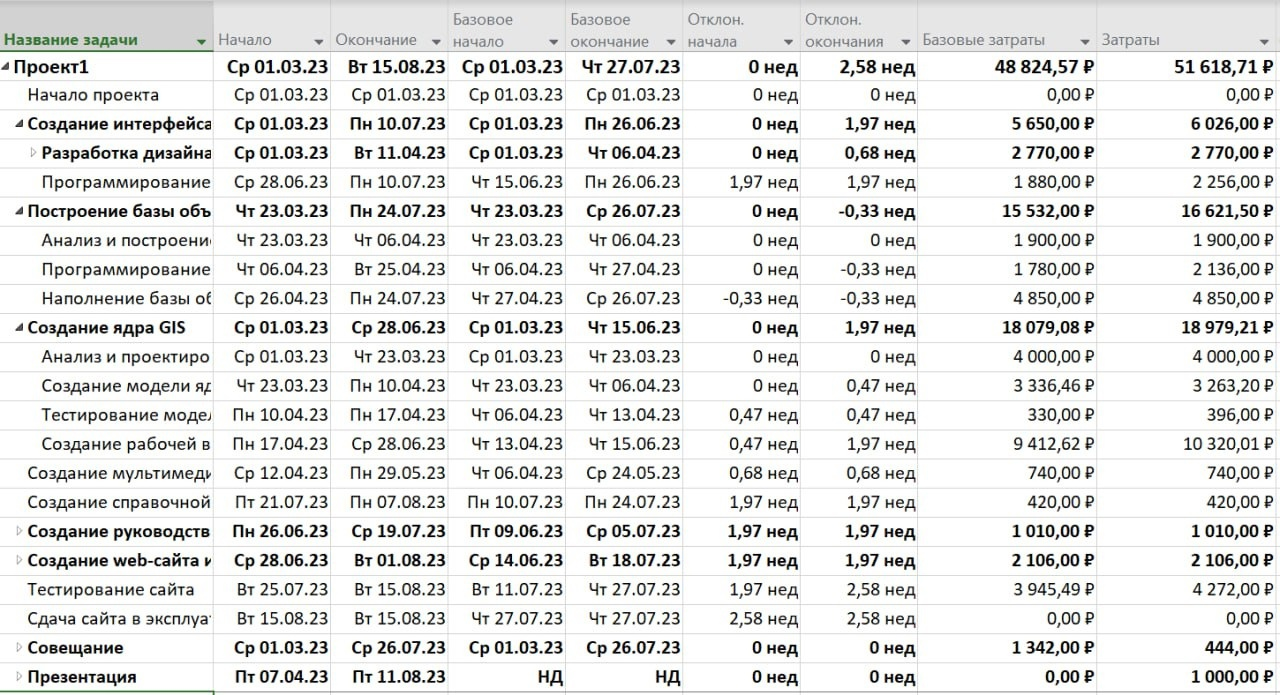
\includegraphics[scale=0.3]{inc/img/deviation1.jpg}
	\end{center}
	\captionsetup{justification=centering}
	\caption{Отклонения от базового плана после актуализации}
	\label{img:deviation1}
\end{figure}

Для снижения отклонений по затратам вместо аренды дополнительного сервера был куплен собственный сервер за 1000 рублей. В результате отклонение по затратам сократилось до 351.04 рублей, как представлено на рисунке~\ref{img:deviation2}. В запасе проекта 824.39 рублей и 16 дней. 

\begin{figure}[H]
	\begin{center}
		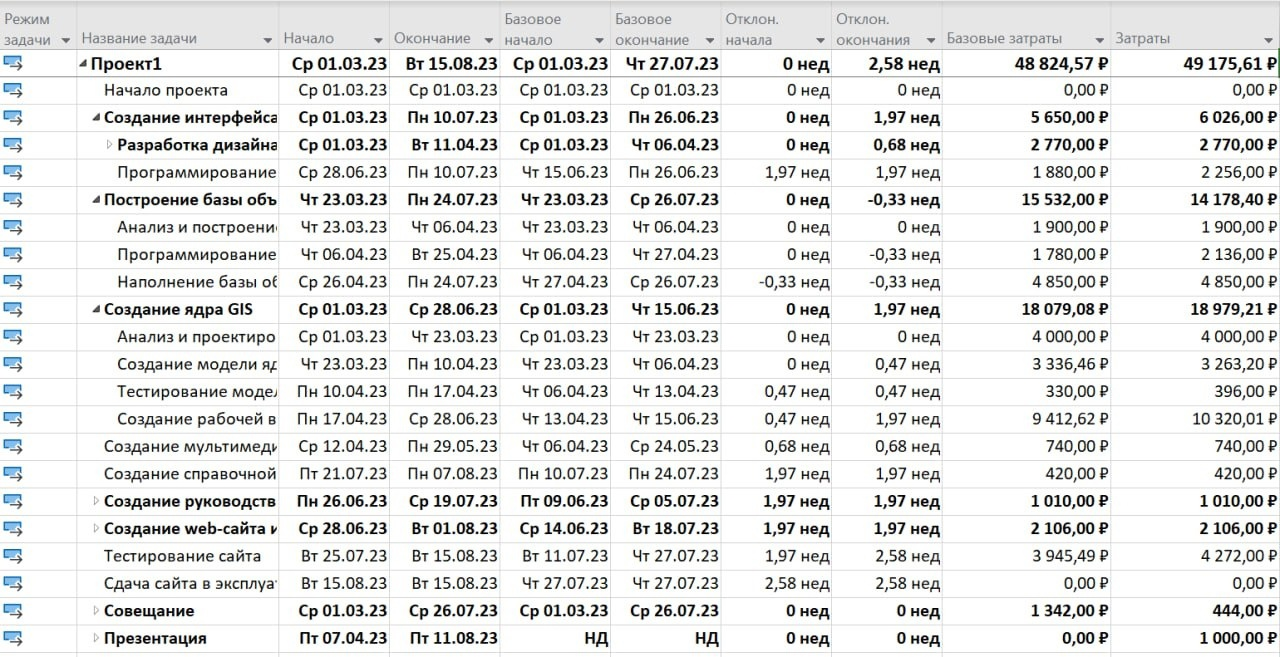
\includegraphics[scale=0.3]{inc/img/deviation2.jpg}
	\end{center}
	\captionsetup{justification=centering}
	\caption{Отклонения от базового плана после покупки собственного сервера}
	\label{img:deviation2}
\end{figure}

\section*{Задание 1}

Согласно таблице затрат, приведенной на рисунках \ref{img:costs1}-\ref{img:costs3}, фактические затраты проекта на дату отчета составляют 25 158.36 рублей.

\begin{figure}[H]
	\begin{center}
		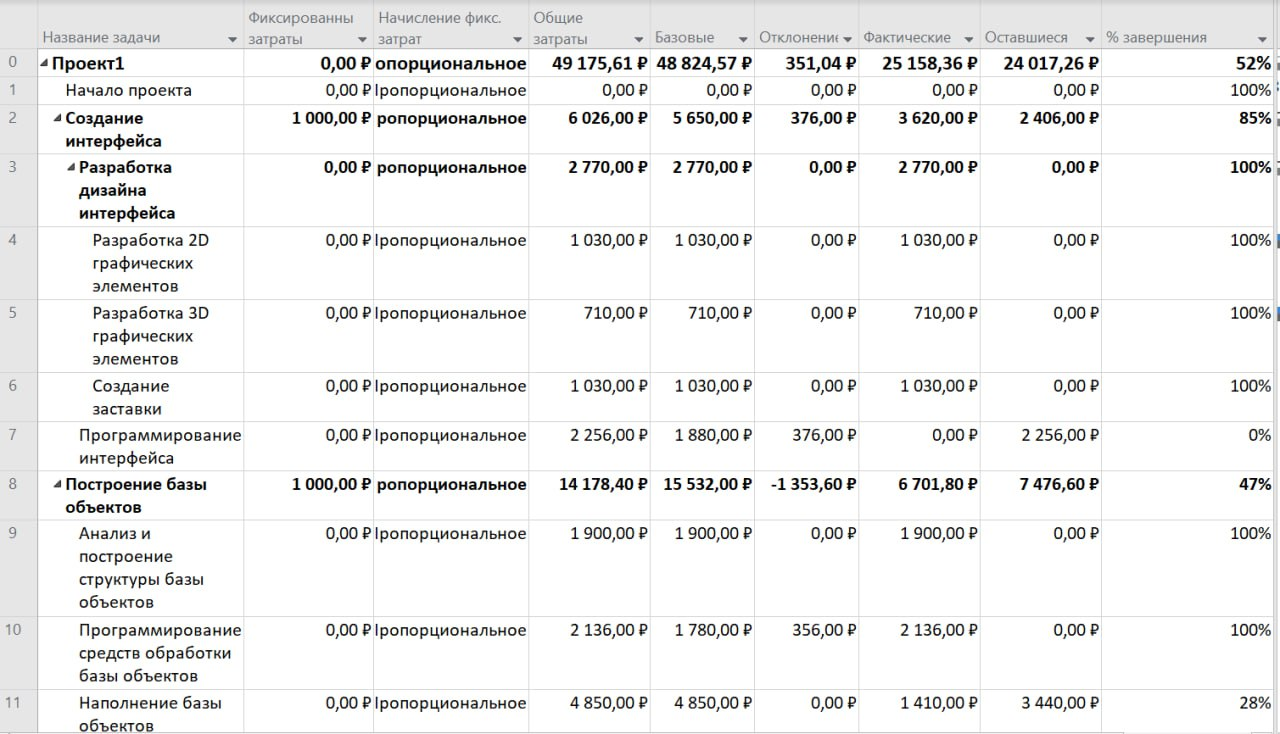
\includegraphics[scale=0.45]{inc/img/costs1.jpg}
	\end{center}
	\captionsetup{justification=centering}
	\caption{Таблица затрат}
	\label{img:costs1}
\end{figure}

\begin{figure}[H]
	\begin{center}
		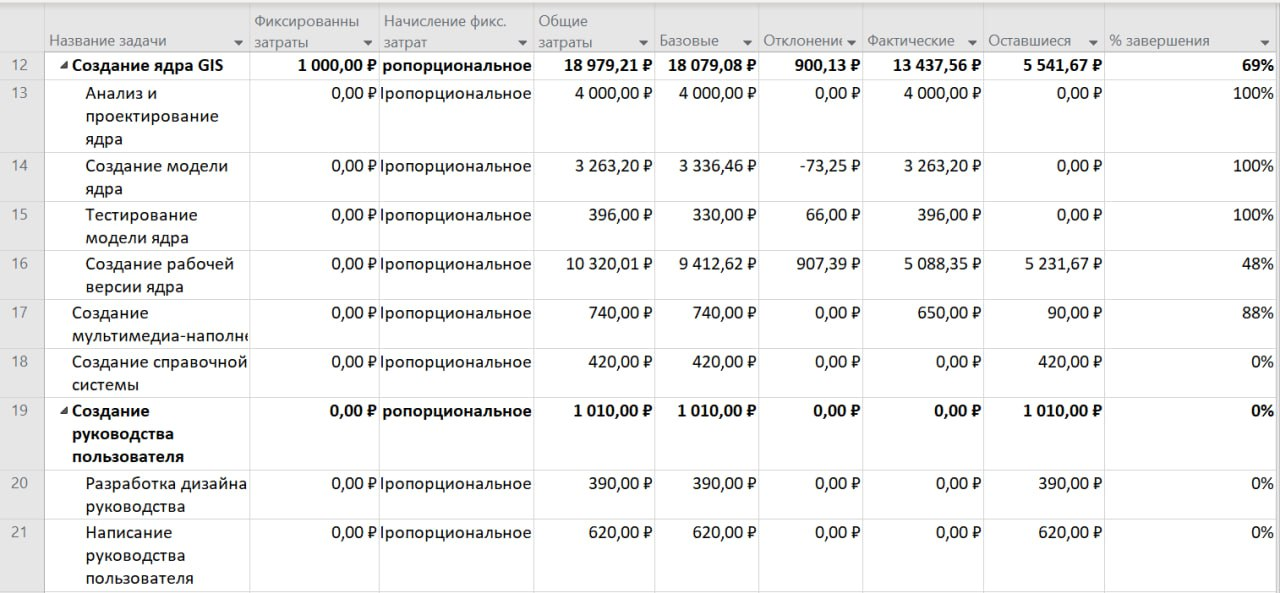
\includegraphics[scale=0.45]{inc/img/costs2.jpg}
	\end{center}
	\captionsetup{justification=centering}
	\caption{Таблица затрат}
	\label{img:costs2}
\end{figure}

\begin{figure}[H]
	\begin{center}
		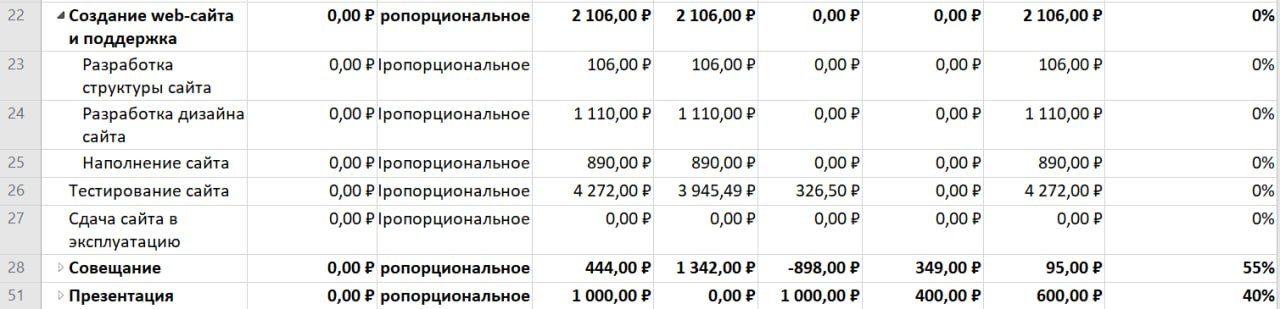
\includegraphics[scale=0.45]{inc/img/costs3.jpg}
	\end{center}
	\captionsetup{justification=centering}
	\caption{Таблица затрат}
	\label{img:costs3}
\end{figure}

Прямые затраты, связанные с выполнением:

\begin{itemize}
	\item задачи <<Создание интерфейса>>, составляют $1000 \cdot 85 \% = 850$ рублей;
	\item задачи <<Построение базы объектов>>, составляют $1000 \cdot 47 \% = 470$ рублей;
	\item задачи <<Создание ядра GIS>>, составляют $1000 \cdot 69 \% = 690$ рублей.
\end{itemize}

Прямые затраты проекта составляют 2010 рублей. Косвенные затраты проекта, связанные с использованием ресурсов, составляют 25 158.36 - 2010 = 23 148.36 рублей. 

В результате анализа таблицы затрат на дату отчета можно сделать следующий вывод: большую часть затрат (около 92\%, прямые затраты составляют около 8\%) составляют затраты, связанные с использованием ресурсов.

Таблица освоенного объема, показанная на рисунках \ref{img:volume1}-\ref{img:volume3}, содержит следующие параметры:

\begin{itemize}
	\item запланированный объем (ЗО) --- те средства, которые были бы затрачены на выполнение задачи в период с начала проекта до выбранной даты отчета, если бы задача точно соответствовала графику и смете;
	\item освоенный объем (ОО) --- те средства, которые были бы затрачены на выполнение задачи с самого начала проекта до выбранной даты отчета, если бы фактически выполненная работа оплачивалась согласно смете, т.е. это фактическое количество рабочих часов, оплачиваемых по сметным ставкам;
	\item фактические затраты (ФЗ) --- средства, фактически потраченные на выполнение задачи в период с начала
проекта до выбранной даты отчета, т.е. это фактическая стоимость задачи или фактическая ставка, умноженная на фактические часы;
	\item отклонение от календарного плана (ОКП = ОО - ЗО) --- сравнивает сметную стоимость плановой и выполненной работы и позволяет вычислить несоответствие сметы, вызванное исключительно различиями между плановым и фактическим объемом работы;
	\item отклонение по стоимости (ОПС = ОО - ФЗ) --- сравнивает сметную и фактическую стоимость выполненной работы и позволяет выделить несоответствие сметы, вызванные разницей стоимости ресурсов;
	\item предварительная оценка по завершении (ПОПЗ) --- ожидаемые общие затраты для задачи, расчет которых основан на предположении, что оставшаяся часть работы будет выполнена в точном соответствии со сметой;
	\item затраты по базовому плану (БПЗ)--- фиксированные затраты и стоимость ресурсов согласно базовому плану;
	\item отклонение по завершению (ОПЗ = БПЗ - ПОПЗ) --- разность между БПЗ и ПОПЗ.
\end{itemize}

\begin{figure}[H]
	\begin{center}
		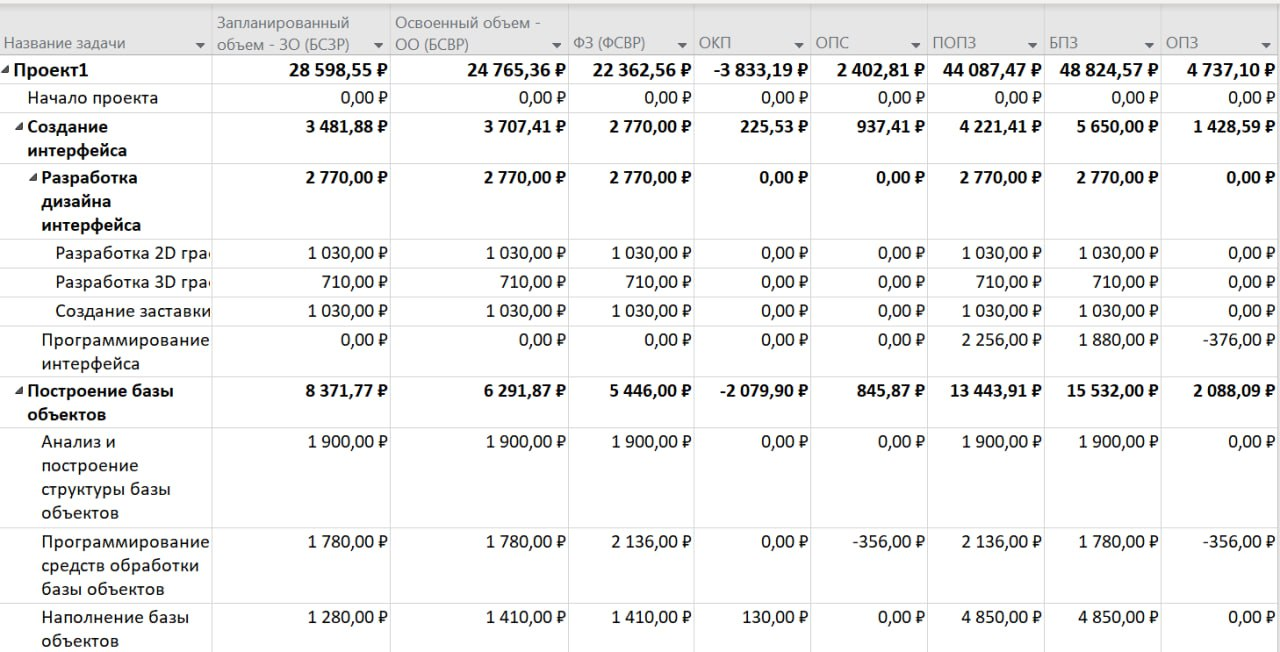
\includegraphics[scale=0.4]{inc/img/volume1.jpg}
	\end{center}
	\captionsetup{justification=centering}
	\caption{Таблица освоенного объема}
	\label{img:volume1}
\end{figure}

\begin{figure}[H]
	\begin{center}
		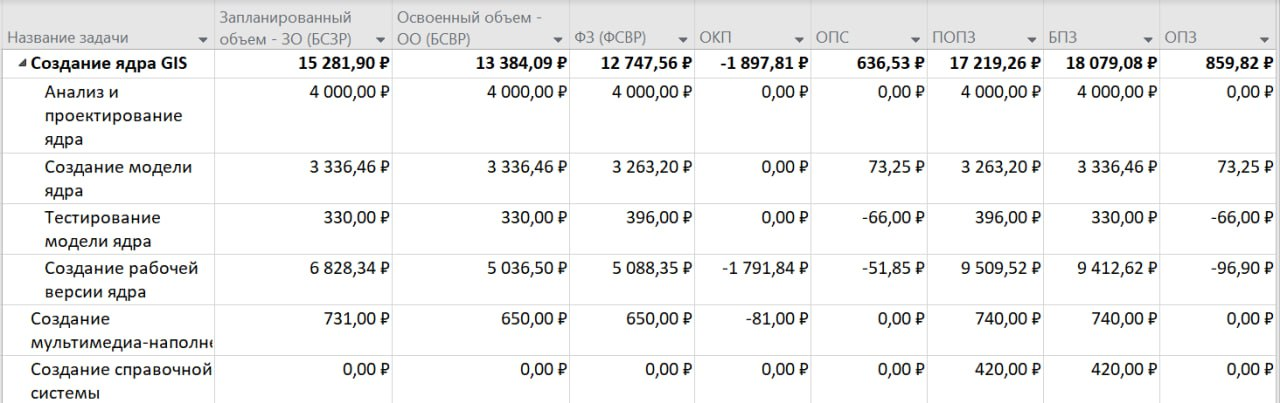
\includegraphics[scale=0.45]{inc/img/volume2.jpg}
	\end{center}
	\captionsetup{justification=centering}
	\caption{Таблица освоенного объема}
	\label{img:volume2}
\end{figure}

\begin{figure}[H]
	\begin{center}
		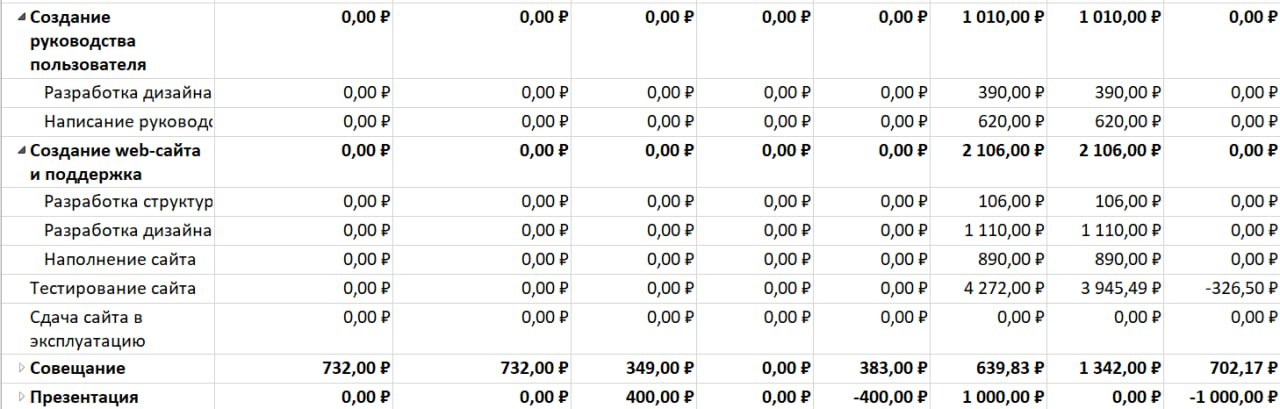
\includegraphics[scale=0.45]{inc/img/volume3.jpg}
	\end{center}
	\captionsetup{justification=centering}
	\caption{Таблица освоенного объема}
	\label{img:volume3}
\end{figure}

В результате анализа таблицы освоенного объема можно сделать следующие выводы:

\begin{itemize}
	\item ОКП < 0 --- проект выполняется с отставанием;
	\item ОПС > 0 --- проект укладывается в смету, за счет этих средств можно выделить дополнительные ресурсы, чтобы ликвидировать отставание;
	\item ОПЗ > 0 --- отсутствует перерасход средств.
\end{itemize}

Отставание проекта произошло по причине увольнения ведущего программиста с 24.03.2023, в связи с чем были увеличены длительности задач по построению базы объектов и созданию ядра GIS, на которые ресурс был назначен. Получено положительное отклонение по стоимости за счет исключения ресурсов с еженедельных совещаний с 1.04.2023 в соответствии с расписанием сотрудников и замены аренды дополнительного сервера на использование собственного.

\section*{Задание 2}

Согласно отчету о бюджетной стоимости, представленному на рисунке \ref{img:budget-report}, руководитель проекта будет испытывать наибольшую потребность в деньгах на 27 неделе года --- с 3.07.2023 по 9.07.2023. На эту неделю приходится выполнение максимального одновременного количества задач: <<Наполнение базы объектов>>, <<Создание мультимедиа-наполнения>>, <<Создание справочной системы>>, <<Написание руководства пользователя>>, <<Наполнение сайта>>. 

\begin{figure}[H]
	\begin{center}
		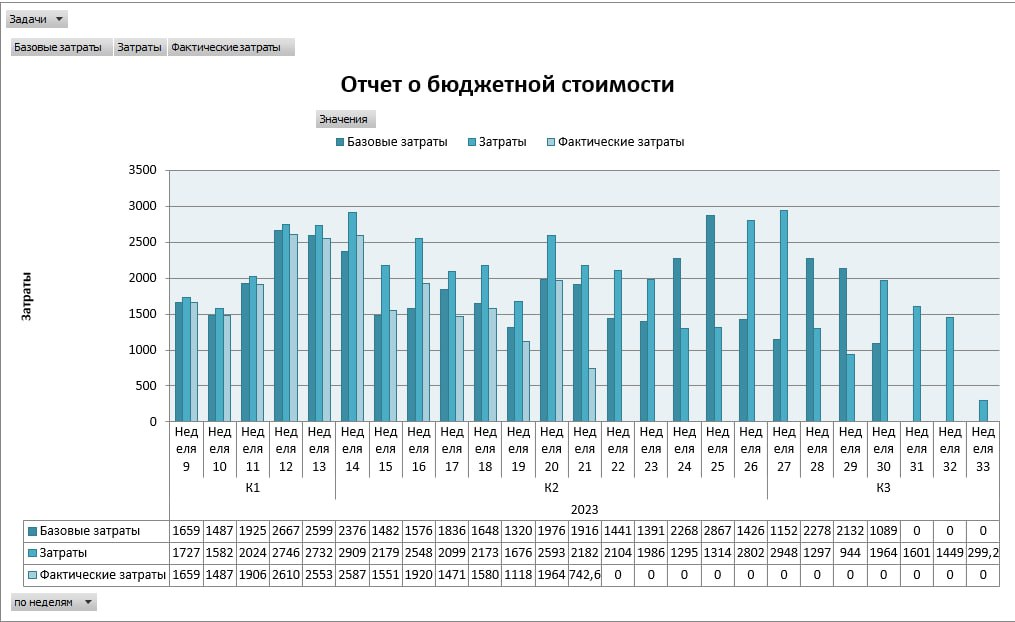
\includegraphics[scale=0.6]{inc/img/budget-report.jpg}
	\end{center}
	\captionsetup{justification=centering}
	\caption{Отчет о бюджетной стоимости}
	\label{img:budget-report}
\end{figure}

Анализ графика и таблицы отклонения по стоимостям для задач, приведенных на рисунках \ref{img:task-graph} и \ref{img:task-table}, показал:

\begin{itemize}
	\item наибольшее превышение стоимости у добавленной с 1.04.2023 повторяющейся задачи <<Презентация>>, так как на каждую презентацию необходима пачка бумаги стоимостью 100 рублей;
	\item положительное отклонение по стоимости для задачи <<Создание ядра GIS>> связано с увеличением с 1.04.2023 заработной платы на 20\% программистам 1-4, выполняющие работы этой задачи;
	\item положительное отклонение по стоимости для задачи <<Тестирование сайта>> связано с увеличением с 1.04.2023 заработной платы на 20\% программистам 1-4, выполняющие работы этой задачи;
	\item положительное отклонение по стоимости для задачи <<Создание интерфейса>> связано с тем, что подзадача <<Создание заставки>> закончилась на пять дней позже;
	\item максимальное уменьшение стоимости у задачи <<Построение базы объектов>>, так как задача <<Программирование средств обработки базы объектов>> закончилась на семь дней раньше, и с даты отчета аренда дополнительного сервера была заменена на покупку собственного сервера;
	\item отрицательное отклонение по стоимости для задачи <<Совещание>> связано с тем, что с 1.04.2023 в еженедельных совещаниях стали принимать участие только те сотрудники, у которых есть задачи на текущей неделе.
\end{itemize}

\begin{figure}[H]
	\begin{center}
		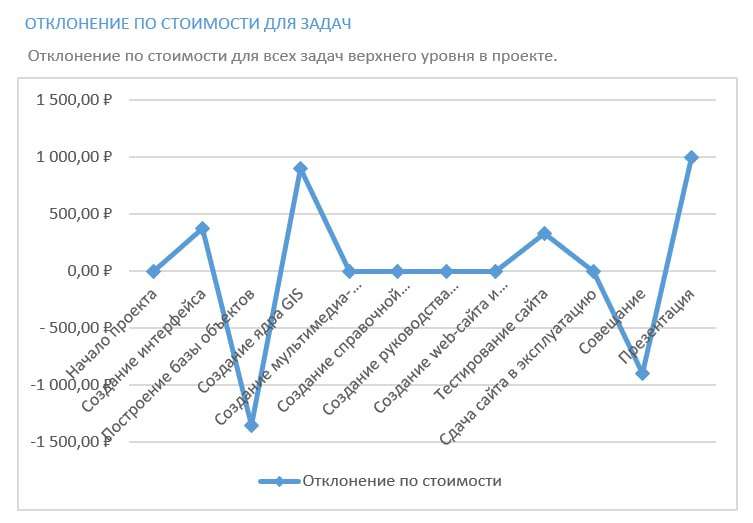
\includegraphics[scale=0.5]{inc/img/task-graph.jpg}
	\end{center}
	\captionsetup{justification=centering}
	\caption{График отклонения по стоимостям для задач}
	\label{img:task-graph}
\end{figure}

\begin{figure}[H]
	\begin{center}
		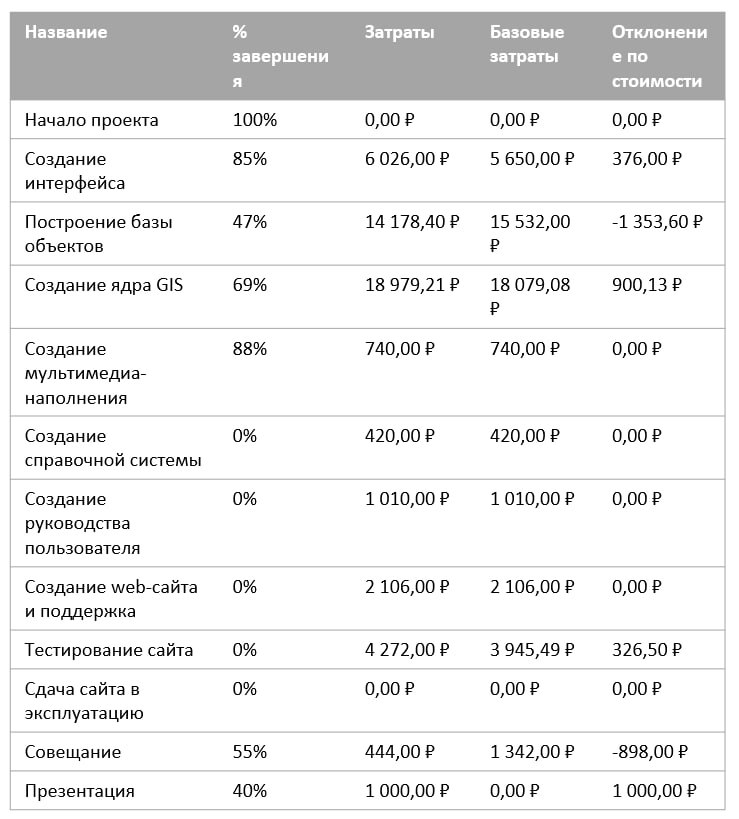
\includegraphics[scale=0.4]{inc/img/task-table.jpg}
	\end{center}
	\captionsetup{justification=centering}
	\caption{Таблица отклонения по стоимостям для задач}
	\label{img:task-table}
\end{figure}

Анализ графика и таблицы отклонения по стоимостям для ресурсов, показанных на рисунках \ref{img:resource-graph} и \ref{img:resource-table}, показал:

\begin{itemize}
	\item увеличение затрат на ресурсы <<Программист 1>>-<<Программист 4>> связано с увеличением с 1.04.2023 их заработной платы на 20\%;
	\item положительное отклонение по стоимости для ресурса <<Бумага>> связано с проведением с 1.04.2023 повторяющейся задачи <<Презентация>>, на которую назначен данный ресурс;
	\item положительное отклонение по стоимости для ресурса <<Собственный сервер>> связано с покупкой собственного сервера за 1000 рублей;
	\item максимальное уменьшение затрат на ресурс <<Ведущий программист>> связано с его увольнением с 24.03.2023;
	\item отрицательное отклонение по стоимости для ресурса <<Сервер>> связано с тем, что с даты отчета аренда данного ресурса была заменена на использование собственного сервера;
	\item отрицательное отклонение по стоимости для ресурсов <<Системный аналитик>>, <<Художник-дизайнер>>, <<Технический писатель>>, <<Web-дизайнер>> и <<3D-аниматор>> связано с тем, что с 1.04.2023 в еженедельных совещаниях стали принимать участие только те сотрудники, у которых есть задачи на текущей неделе.
\end{itemize}

\begin{figure}[H]
	\begin{center}
		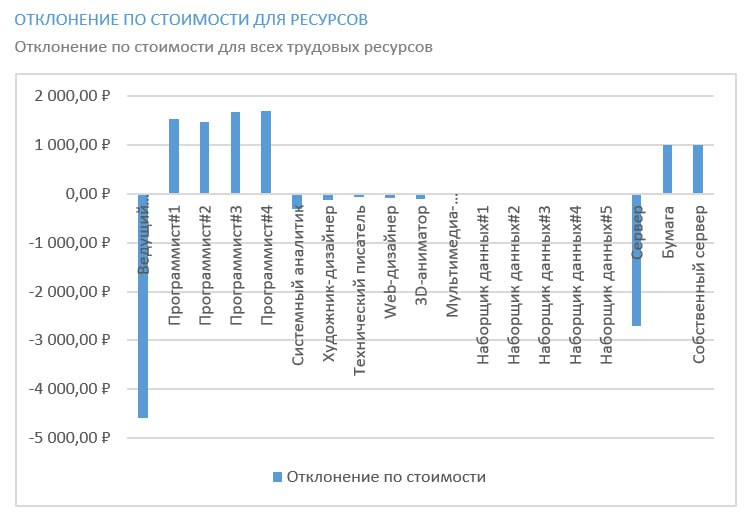
\includegraphics[scale=0.5]{inc/img/resource-graph.jpg}
	\end{center}
	\captionsetup{justification=centering}
	\caption{График отклонения по стоимостям для ресурсов}
	\label{img:resource-graph}
\end{figure}

\begin{figure}[H]
	\begin{center}
		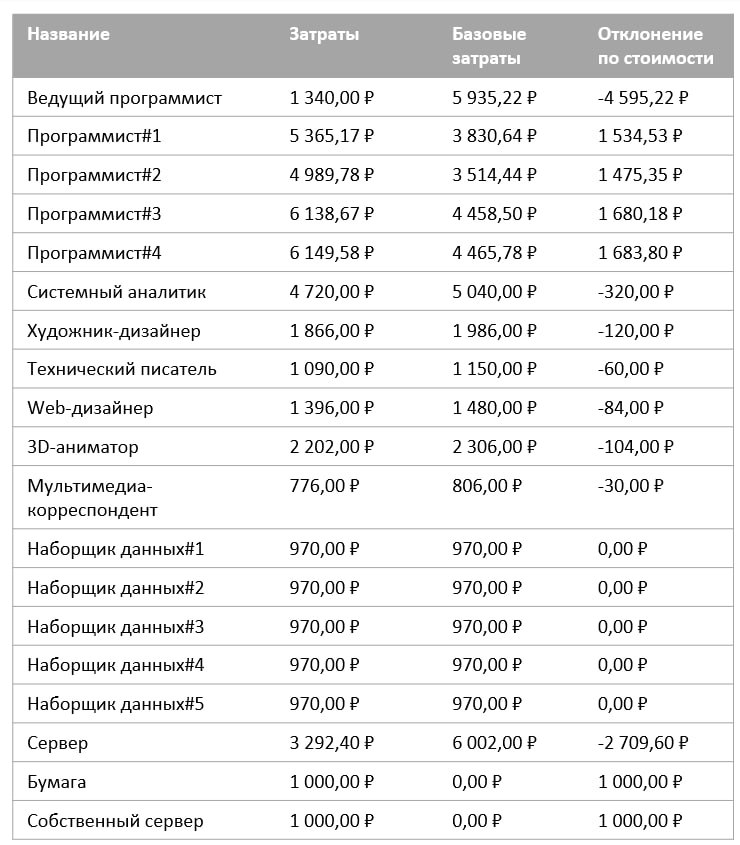
\includegraphics[scale=0.4]{inc/img/resource-table.jpg}
	\end{center}
	\captionsetup{justification=centering}
	\caption{Таблица отклонения по стоимостям для ресурсов}
	\label{img:resource-table}
\end{figure}
 
\section*{Задание 3}

На рисунке \ref{img:lab2} представлена полученная в результате выполнения лабораторной работы № 2 декомпозиция проекта.

\begin{figure}[H]
	\begin{center}
		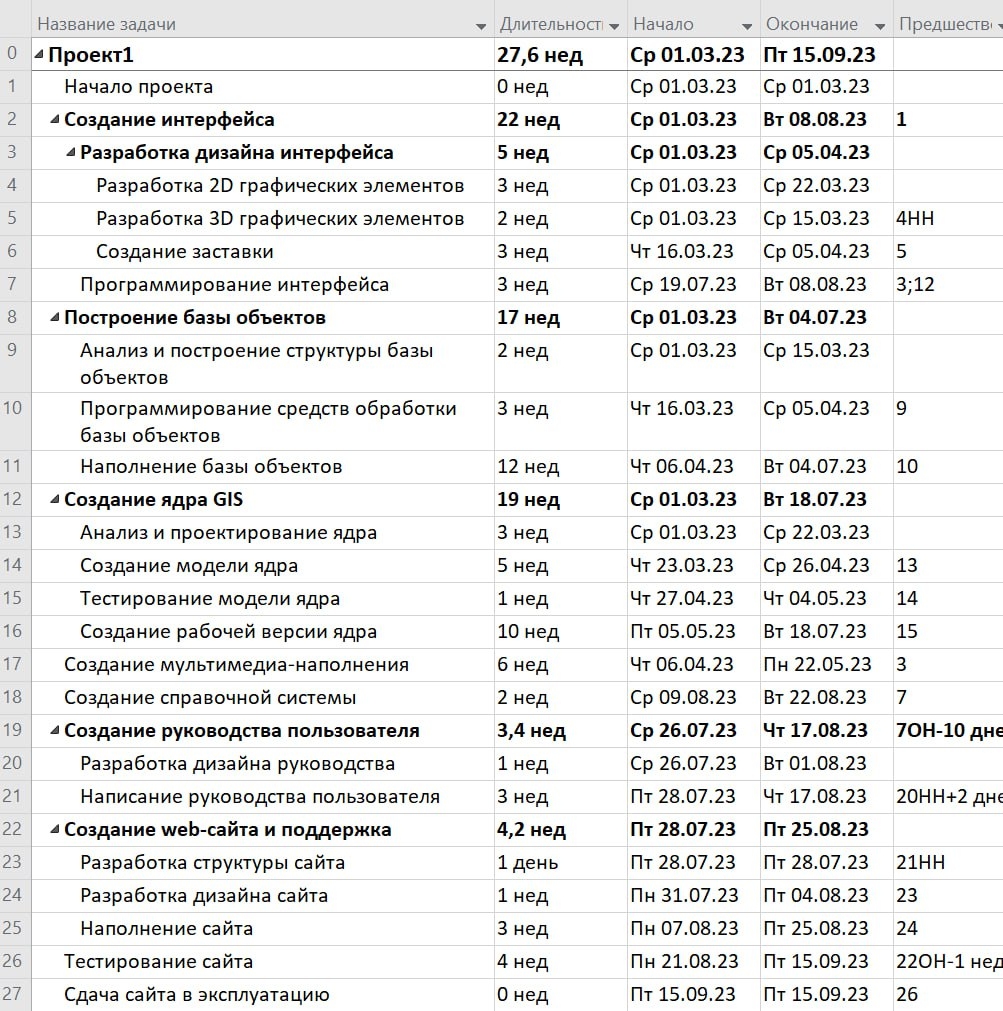
\includegraphics[scale=0.35]{inc/img/lab2.jpg}
	\end{center}
	\captionsetup{justification=centering}
	\caption{Полученная в результате выполнения лабораторной работы № 2 декомпозиция проекта}
	\label{img:lab2}
\end{figure}

При декомпозиции проекта, полученной в результате выполнения лабораторной работы № 2, проект оканчивается 15.09.2023, его затраты составляют 48 094 рублей. Проект укладывается в бюджет, но не укладывается в заявленный срок выполнения.

Для проведения новой декомпозиции были выделены следующие этапы проекта:

\begin{itemize}
	\item анализ и проектирование;
	\item создание:
		\begin{itemize}
			\item разработка;
			\item кодирование;
			\item наполнение;
		\end{itemize}
	\item документирование;
	\item тестирование.
\end{itemize}

После установления связей между задачами, назначения фиксированных затрат и сервера задачам была получена декомпозиция, приведенная на рисунке \ref{img:new-decomposition}. Затраты и трудозатраты показаны на рисунке \ref{img:stat1}.

\begin{figure}[H]
	\begin{center}
		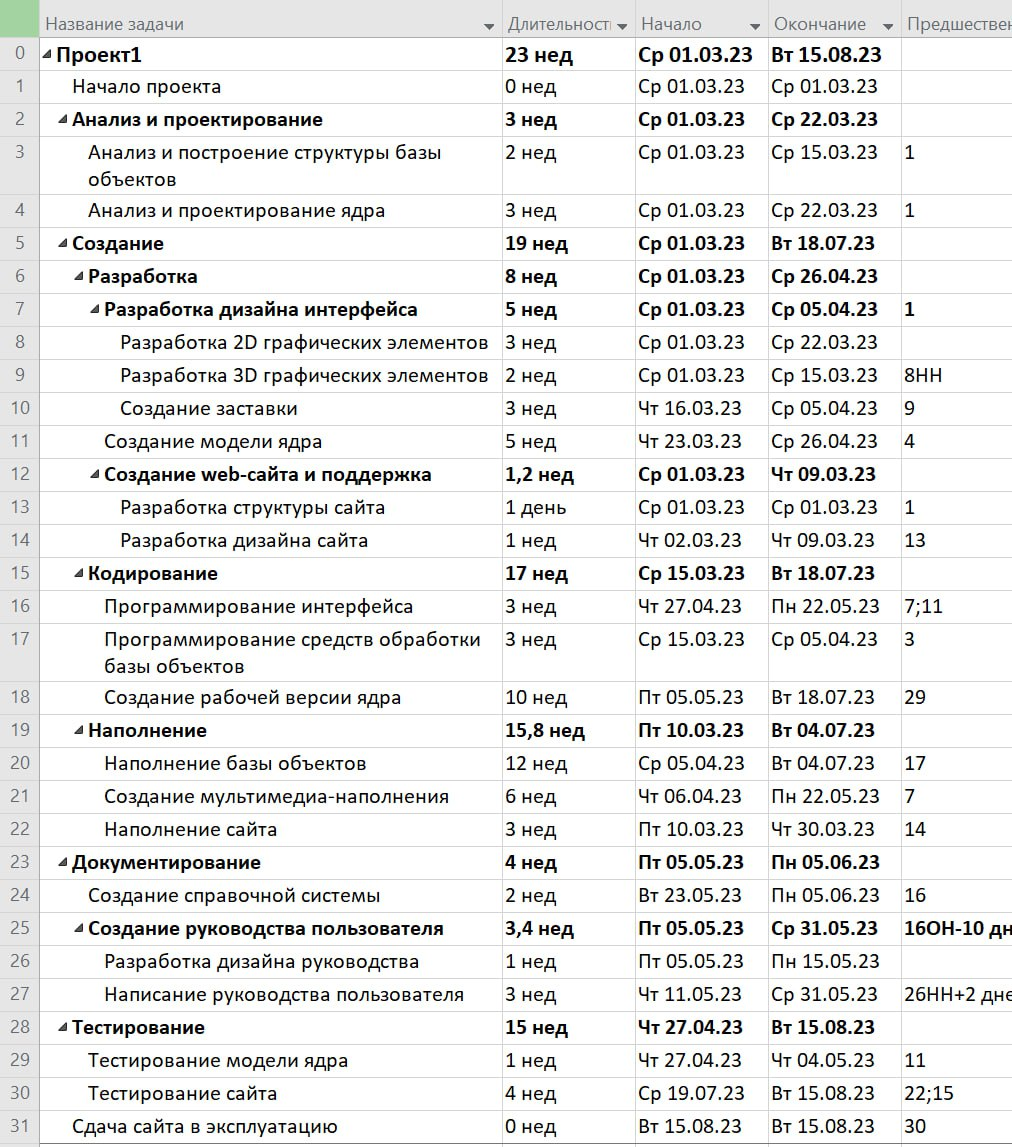
\includegraphics[scale=0.3]{inc/img/new-decomposition.jpg}
	\end{center}
	\captionsetup{justification=centering}
	\caption{Новая декомпозиция проекта}
	\label{img:new-decomposition}
\end{figure}

\begin{figure}[H]
	\begin{center}
		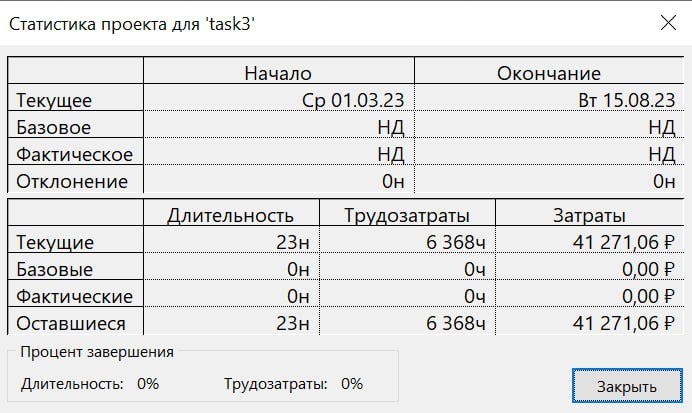
\includegraphics[scale=0.4]{inc/img/stat1.jpg}
	\end{center}
	\captionsetup{justification=centering}
	\caption{Затраты и трудозатраты при новой декомпозиции проекта}
	\label{img:stat1}
\end{figure}

При новой декомпозиции проект завершается на месяц раньше --- 15.08.2023, его затраты снижаются до 41 271.06 рублей. Длительность проекта уменьшилась в связи с началом создания web-сайта с началом проекта и началом программирования интерфейса после создания модели ядра. Уменьшение затрат связано с сокращением времени работы сервера за счет исключения его с задачи <<Анализ и построение структуры базы объектов>>.

На рисунке \ref{img:lab3} представлен результат оптимизации затрат и критического пути проекта, полученный при выполнении лабораторной работы № 3. Статистика проекта приведена на рисунке \ref{img:lab3-stat}.

\begin{figure}[H]
	\begin{center}
		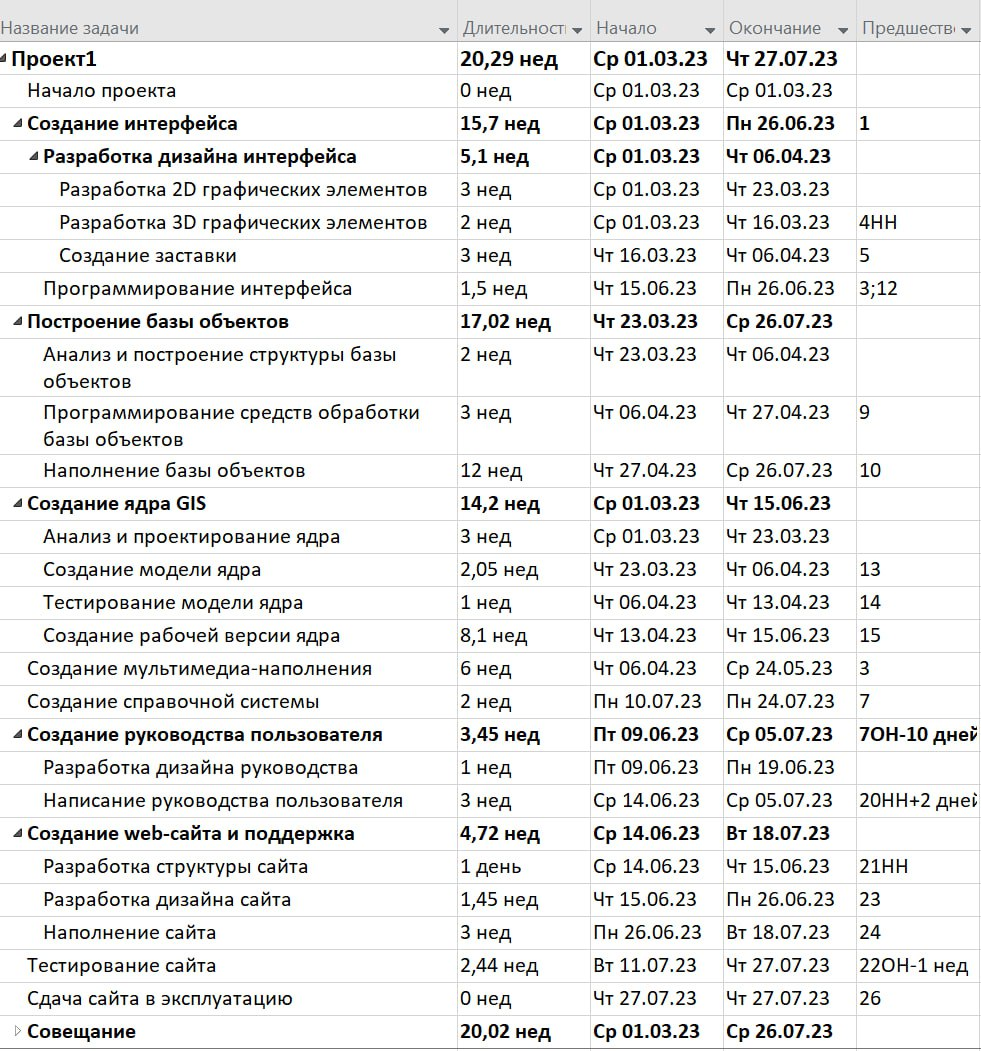
\includegraphics[scale=0.3]{inc/img/lab3.jpg}
	\end{center}
	\captionsetup{justification=centering}
	\caption{Результат оптимизации затрат и критического пути проекта (лабораторная работа № 3)}
	\label{img:lab3}
\end{figure}

\begin{figure}[H]
	\begin{center}
		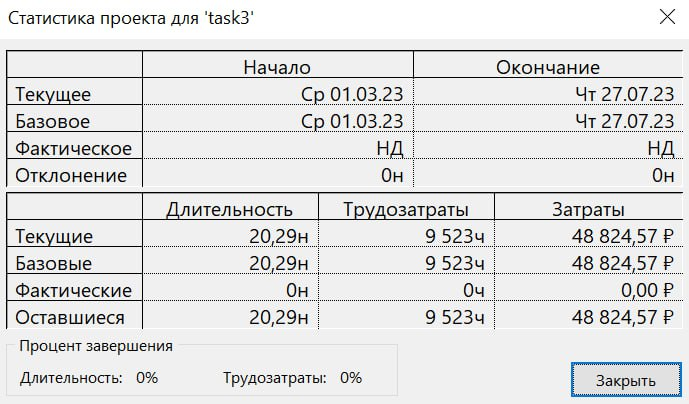
\includegraphics[scale=0.4]{inc/img/lab3-stat.jpg}
	\end{center}
	\captionsetup{justification=centering}
	\caption{Статистика проекта}
	\label{img:lab3-stat}
\end{figure}

В проекте, построенном по новой декомпозиции, были проведены оптимизация затрат --- сокращение затрат на использование сотрудников, которые не использовали свои рабочие места во время совещаний, и оптимизация критического пути --- назначение всех программистов на все задачи, связанные с программированием. Полученный результат показан на рисунке \ref{img:result}. Статистика проекта представлена на рисунке \ref{img:result-stat}.

\begin{figure}[H]
	\begin{center}
		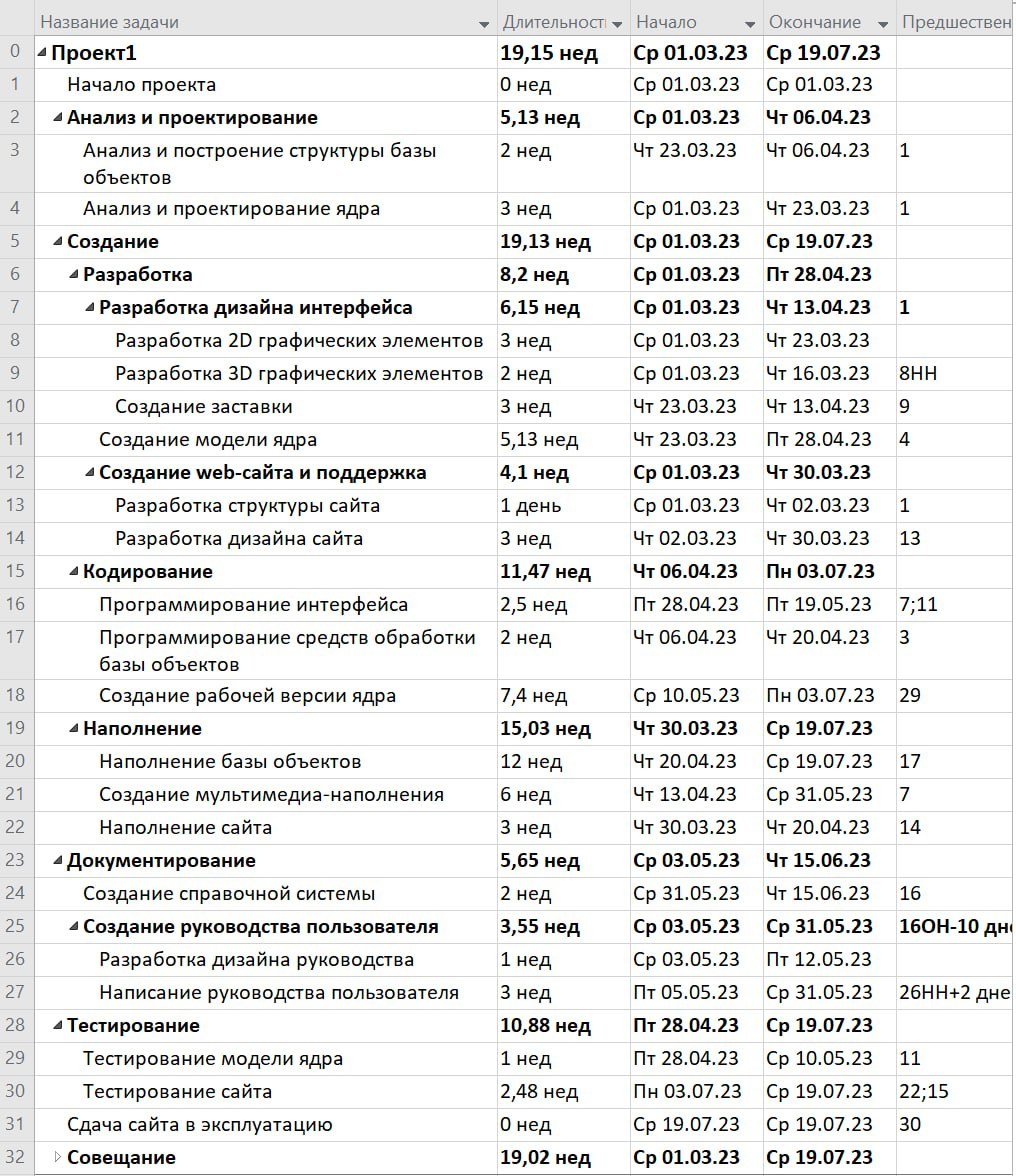
\includegraphics[scale=0.3]{inc/img/result.jpg}
	\end{center}
	\captionsetup{justification=centering}
	\caption{Результат оптимизации затрат и критического пути проекта с новой декомпозицией}
	\label{img:result}
\end{figure}

\begin{figure}[H]
	\begin{center}
		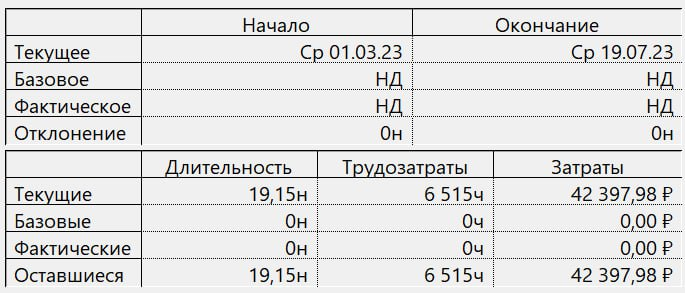
\includegraphics[scale=0.45]{inc/img/result-stat.jpg}
	\end{center}
	\captionsetup{justification=centering}
	\caption{Статистика проекта}
	\label{img:result-stat}
\end{figure}

При новой декомпозиции дата завершения проекта сдвинулась с 27.07.2023 на 19.07.2023, затраты снизились с 48 824.57 рублей до 42 397.98 рублей.

\section*{Вывод}

При выполнении лабораторной работы были отработаны навыки использования программы Microsoft Project для управления финансовыми потоками на основе анализа затрат.

По методу освоенного объема было определено, что проект выполняется с отставанием, однако укладывается в смету, при этом отсутствует перерасход средств, что позволяет ликвидировать отставание.

Работа с отчетами позволяет проследить движение средств в проекте. Из отчета о бюджетной стоимости стало понятно, что руководитель проекта будет испытывать наибольшую потребность в деньгах на 27 неделе года.

Введение новой декомпозиции позволило сократить длительность и затраты проекта.
